\documentclass[aspectratio=169]{beamer}
\usepackage[T1]{fontenc}
\usepackage[utf8]{inputenc}
\usepackage[ngerman]{babel}
\usepackage{amsmath,amssymb}
\usepackage{booktabs}
\usepackage{graphicx}
\usepackage{xcolor}

\usetheme{Madrid}
\usecolortheme{default}
\setbeamertemplate{navigation symbols}{}

\definecolor{tuwblue}{RGB}{0,102,153}
\setbeamercolor{structure}{fg=tuwblue}
\setbeamercolor{title}{fg=white,bg=tuwblue}
\setbeamercolor{frametitle}{fg=white,bg=tuwblue}

\setbeamersize{text margin left=5mm, text margin right=5mm}

\title{Hess-Smith Panelverfahren}
\subtitle{Präsentationstechniken in der Physik}
\author{Sebastian Matkovich}
\institute{TU Wien}
\date{2026}

% Trim values: left bottom right top — removes MATLAB whitespace
\newcommand{\plotimg}[1]{\includegraphics[width=\textwidth,height=2.8cm,keepaspectratio]{#1}}
\newcommand{\plotimgbig}[1]{\includegraphics[width=\textwidth,height=5.2cm,keepaspectratio]{#1}}

\begin{document}

\begin{frame}
  \titlepage
\end{frame}

%=== FOLIE 1: Grundlagen ===
\begin{frame}{Grundlagen -- Von den Annahmen zur Laplace-Gleichung}
\footnotesize

\begin{columns}[T]
\begin{column}{0.48\textwidth}
\textbf{Annahmen:} ebene, stationäre, inkompressible, reibungsfreie Strömung.

\smallskip
Reibungsfrei $\Rightarrow$ \textbf{wirbelfrei} (Helmholtz):
$\;\nabla\times\vec{v}=0$
\;\;$\Rightarrow$ Geschwindigkeitspotential existiert:
$\;\vec{v} = \nabla\varphi$

Einsetzen in die Kontinuitätsgleichung ($\nabla\cdot\vec{v}=0$):
\vspace{-2mm}
\[
  \nabla\cdot\vec{v} = 0
  \quad\xrightarrow{\;\vec{v}=\nabla\varphi\;}
  \quad\underbrace{\nabla\cdot(\nabla\varphi)}_{\text{div(grad}\,\varphi)} = \Delta\varphi = 0
\]

\vspace{-3mm}
Das ist die \textbf{Laplace-Gleichung}.
Weil sie \textbf{linear} ist, erfüllt jede Überlagerung
von Elementarlösungen sie ebenfalls.
$\to$ Kontur in $n$ \textbf{Panele} unterteilen, auf jedem
Quellen ansetzen -- $\Delta\varphi=0$ automatisch
erfüllt, nur die Randbedingung bleibt.
\end{column}
\begin{column}{0.48\textwidth}
\textbf{Elementarlösung} -- radialsymmetrischer Ansatz
$\varphi(r)$. Laplace in Polarkoordinaten ohne $\theta$:
\vspace{-1mm}
\[
  \frac{1}{r}\frac{d}{dr}\!\left(r\frac{d\varphi}{dr}\right) = 0
\]

\vspace{-2mm}
Integrieren: $\;r\,\varphi' = C_1$, also $\;\varphi' = C_1/r$.
Nochmal: $\;\varphi = C_1 \ln r + C_2$.

\smallskip
$C_1$ folgt aus der Quellstärke~$m$
(Volumenstrom durch jeden Kreis $= m$):
\vspace{-1mm}
\[
  \oint \vec{v}\!\cdot\!\hat{n}\;ds = 2\pi\, C_1 \stackrel{!}{=} m
  \;\;\Rightarrow\;\;
  C_1 = \tfrac{m}{2\pi}
\]

\vspace{-2mm}
\textbf{Ergebnis} -- Punktquelle mit Stärke $m$:
\vspace{-1mm}
\[
  \boxed{\varphi = \frac{m}{2\pi}\ln r\,,
  \qquad
  \vec{v} = \frac{m}{2\pi r}\,\hat{e}_r}
\]
\end{column}
\end{columns}

\end{frame}

%=== FOLIE 2: Quellbelegung & cp ===
\begin{frame}{Quellbelegung und Druckbeiwert $c_p$}
\footnotesize

\begin{columns}[T]
\begin{column}{0.48\textwidth}
\textbf{Quellbelegung (ohne Wirbel):}

\smallskip
Auf jedem Panel sitzt eine \textbf{konstante Quellverteilung}~$q_j$
(Fluidausstoß pro Längeneinheit -- mathematischer Trick).

\smallskip
Die Geschwindigkeit am Mittelpunkt von Panel~$i$ setzt sich
zusammen aus der Anströmung~$V_\infty$ und den Beiträgen
\emph{aller} Panels. Integration der Punktquell-Beiträge über
jedes Panel liefert \textbf{Einflusskoeffizienten}~$M_{i,j}$.

\smallskip
\textbf{Undurchlässigkeitsbedingung} -- die Normalkomponente
der Gesamtgeschwindigkeit muss auf der Oberfläche verschwinden:
\vspace{-1mm}
\[
  \underbrace{\sum_j M_{i,j}\, q_j}_{\text{Panelbeiträge}}
  = \underbrace{-V_\infty\sin(\alpha-\theta_i)}_{\text{Anströmung (normal)}}
  \;\;\Longleftrightarrow\;\;
  M\,\vec{q}=\vec{b}
\]

\vspace{-3mm}
Zunächst \emph{nur Quellen} (kein Auftrieb)
$\to$ Validierung am \textbf{Kreiszylinder}.
\end{column}
\begin{column}{0.48\textwidth}
\textbf{Herleitung des Druckbeiwerts $c_p$:}

\smallskip
Aus den $q_j$ erhält man die Tangentialgeschwindigkeit~$v_t$
an jedem Panel. Bernoulli entlang einer Stromlinie zwischen
ungestörter Anströmung ($\infty$) und Oberfläche:
\[
  p_\infty + \tfrac{1}{2}\rho\, V_\infty^2
  \;=\;
  p + \tfrac{1}{2}\rho\, v_t^2
\]

\vspace{-3mm}
Umstellen nach der Druckdifferenz:
\[
  p - p_\infty = \tfrac{1}{2}\rho\bigl(V_\infty^2 - v_t^2\bigr)
\]

\vspace{-3mm}
Normieren auf den dynamischen Druck $\tfrac{1}{2}\rho V_\infty^2$:
\[
  \boxed{c_p \;=\; \frac{p - p_\infty}{\tfrac{1}{2}\rho\,V_\infty^2}
  \;=\; 1 - \left(\frac{v_t}{V_\infty}\right)^{\!2}}
\]

\vspace{-3mm}
$c_p=1$: Staupunkt ($v_t\!=\!0$) \quad $c_p<0$: Sog ($v_t\!>\!V_\infty$)
\end{column}
\end{columns}

\end{frame}

%=== FOLIE 3: Kreiszylinder ===
\begin{frame}{Validierung am Kreiszylinder}
\footnotesize

\begin{columns}[T]
\begin{column}{0.57\textwidth}
Analytische Lösung (Parallelströmung + Dipol):
\vspace{-1mm}
\[
  v_t = -2V_\infty\sin\varphi
  \;\;\Longrightarrow\;\;
  c_p = 2\cos(2\varphi)-1
\]

\vspace{-3mm}
\begin{itemize}\setlength\itemsep{1pt}
  \item $\varphi\!=\!0^\circ$ (vorne): Staupunkt, $v_t\!=\!0$, $c_p\!=\!1$
  \item $\varphi\!=\!90^\circ$ (Scheitel): $v_t\!=\!2V_\infty$, $c_p\!=\!-3$
  \item $\varphi\!=\!180^\circ$ (hinten): Fluid verzögert sich
        \emph{symmetrisch} $\to$ zweiter Staupunkt, $c_p\!=\!1$
\end{itemize}

\smallskip
Der zweite Staupunkt existiert nur in der reibungsfreien
Potentialströmung.

\smallskip
\textbf{D'Alembertsches Paradoxon:}
Symmetrische Druckverteilung $\Rightarrow$ kein Widerstand.
Real: Grenzschichtablösung $\to$ $c_p<1$ hinten.

\smallskip
\textbf{Konvergenz:} $e\propto n^{-1}$ (Ordnung $p\!=\!1$).
\end{column}
\begin{column}{0.40\textwidth}
  \vspace{-1mm}
  \plotimg{crop_005.png}
  \vspace{-1mm}
  {\tiny\centering 8 Panels -- grobe Näherung\par}
  \vspace{2mm}
  \plotimg{crop_006.png}
  \vspace{-1mm}
  {\tiny\centering 32 Panels -- nahe an analytischer Lösung\par}
\end{column}
\end{columns}

\end{frame}

%=== FOLIE 4: Tragflächenprofile ===
\begin{frame}{Tragflächenprofile -- Symmetrie und Auftrieb}
\footnotesize

\begin{columns}[T]
\begin{column}{0.57\textwidth}
Für Auftrieb: Zusätzlich zu den Quellen wird eine über alle
Panels \textbf{konstante Wirbelbelegung}~$\gamma$ eingeführt.
Das LGS erweitert sich um eine Dimension ($n\!+\!1$ Gleichungen),
die zusätzliche Gleichung ist die \textbf{Kutta-Bedingung}:
gleiche Geschwindigkeitsbeträge an Ober- und Unterseite
der Hinterkante. Der \textbf{Auftriebsbeiwert} ergibt sich aus
der Integration der Druckdifferenz entlang der Sehne:
\vspace{-1mm}
\[
  c_a = \frac{1}{t}\sum_i (c_{p,\text{unten}} - c_{p,\text{oben}})\,\Delta x_i
\]

\vspace{-3mm}
\textbf{NACA\,0012} (sym., $\alpha\!=\!0^\circ$):
ident.\ $c_p$ oben/unten $\to$ $c_a\!=\!0$

\smallskip
\textbf{Eppler\,193} (gewölbt, $\alpha\!=\!0^\circ$):
Sog oben ($c_p\!<\!0$), höherer Druck unten
$\to$ $c_a = 0{,}378$

\smallskip
Bei $\alpha\!\neq\!0^\circ$ erzeugt auch NACA\,0012 Auftrieb.
\end{column}
\begin{column}{0.40\textwidth}
  \vspace{-1mm}
  \begin{minipage}[t]{0.38\textwidth}
    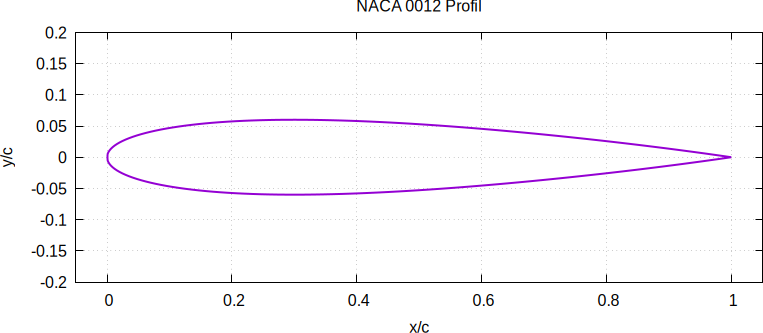
\includegraphics[width=\textwidth]{crop_004.png}
  \end{minipage}\hfill
  \begin{minipage}[t]{0.58\textwidth}
    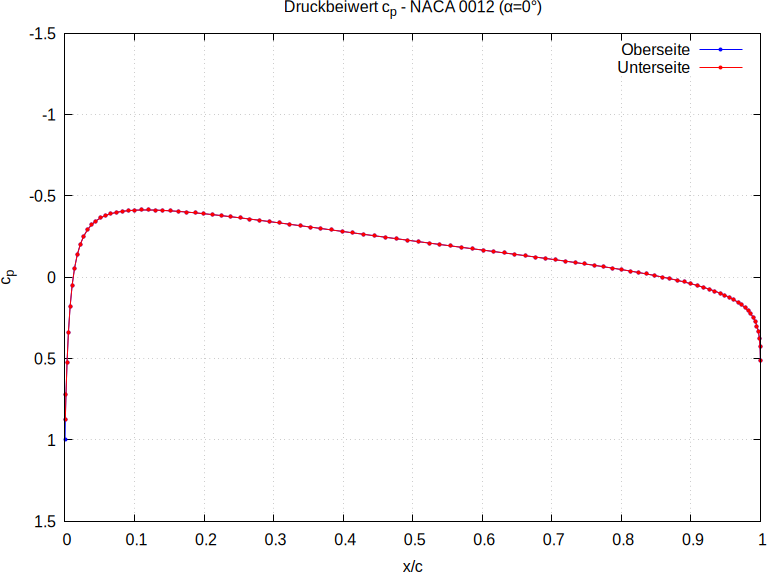
\includegraphics[width=\textwidth]{crop_007.png}
  \end{minipage}
  \vspace{-1mm}
  {\tiny\centering NACA\,0012: symmetrisch $\to$ Kurven deckungsgleich $\to$ $c_a\!=\!0$\par}
  \vspace{1.5mm}
  \begin{minipage}[t]{0.38\textwidth}
    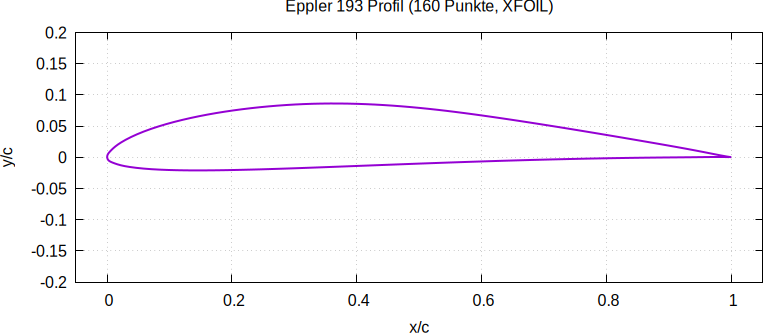
\includegraphics[width=\textwidth]{crop_002.png}
  \end{minipage}\hfill
  \begin{minipage}[t]{0.58\textwidth}
    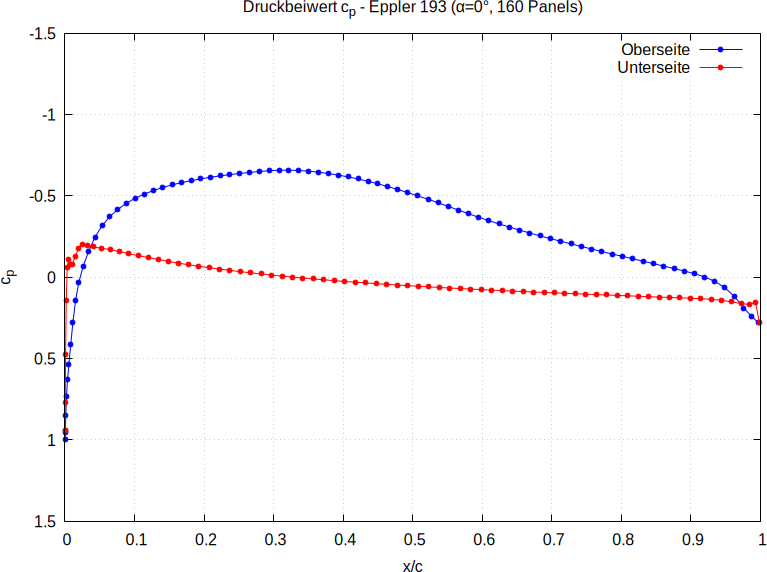
\includegraphics[width=\textwidth]{crop_008.png}
  \end{minipage}
  \vspace{-1mm}
  {\tiny\centering Eppler\,193: gewölbt $\to$ Asymmetrie $\to$ $c_a\!=\!0{,}378$\par}
\end{column}
\end{columns}

\end{frame}

%=== FOLIE 5: XFOIL-Validierung ===
\begin{frame}{Validierung mit XFOIL}
\footnotesize

\begin{columns}[T]
\begin{column}{0.57\textwidth}
Referenz: \textbf{XFOIL} (M.~Drela, MIT) -- Panelmethode mit
\emph{linear variierender} Wirbelbelegung.

\smallskip
\textbf{NACA\,0012} -- Abweichung $< 0{,}15\,\%$:

\vspace{1mm}
{\scriptsize
\begin{tabular}{@{}cccc@{}}
  \toprule
  $\alpha$ & $c_a$ (H-S) & $c_a$ (XFOIL) & Abw. \\
  \midrule
  $0^\circ$  & 0{,}0000 & 0{,}0000 & --      \\
  $5^\circ$  & 0{,}6027 & 0{,}6033 & 0{,}11\,\% \\
  $10^\circ$ & 1{,}2007 & 1{,}2020 & 0{,}11\,\% \\
  \bottomrule
\end{tabular}}

\smallskip
\textbf{Eppler-Profile} -- Abweichung 4--10\,\%:
\begin{itemize}\setlength\itemsep{0pt}
  \item H-S: \emph{konstante} Singularitäten pro Panel
  \item XFOIL: \emph{linear variierende} Wirbelbelegung
  \item Endliche Hinterkantendicke $\to$ Schließungspanel
\end{itemize}
\end{column}
\begin{column}{0.40\textwidth}
  \vspace{-1mm}
  \plotimg{crop_010.png}
  \vspace{-1mm}
  {\tiny\centering NACA\,0012: nahezu deckungsgleich\par}
  \vspace{2mm}
  \plotimg{crop_011.png}
  \vspace{-1mm}
  {\tiny\centering Eppler\,193: sichtbare Abweichung (4--8\,\%)\par}
\end{column}
\end{columns}

\end{frame}

\end{document}
